\documentclass[titlepage]{article}
\usepackage[left=15mm,right=15mm,top=1in,bottom=1in]{geometry}
\usepackage{graphicx}
\graphicspath{ {C:\Users\Nick\Documents\GitHub\3A04\3AO4\doc\intermediateFiles} }
\begin{document}
\title{Stone Identification App \\
	Software Requirements Specification}
\author{Genevieve Okon (Okong), Sydney Lieng(),\\
	Niko Savas(), Nick Lago(lagond),\\
	Eric Le Fort(leforte)}
\date{\today}
\maketitle



\section{Overall Description}
The following section will outline the factors that affect our product and its requirements.\\

\subsection{Product Perspective}
The stone identification app will provide similar functions to rock identification sites, presented in an app to be more accessible and portable. The application will also implement some extra features such as value approximation and marketplaces. The application will work by asking multiple questions to refine the list of rocks suggested by the application. The product will make use of google maps and therefore will not be completely self contained. 
There is no larger system that will be interacting with our application.\\

\subsubsection{Product Functions}
\begin{itemize}

\item If the user finds a rock, the application will display a list of all possible rocks for a match \\
\item Each rock possibility is accompanied by a picture, a description and an approximate value\\
\item The application will display a set of questions as a form that the user can answer to refine the selection of possible rocks\\
\item Once a match has been found, the customer has the option to save rock information to their \"rocks found\" list.\\
\item Customers will be able to remove rocks from their collection\\



\end{itemize}

\subsubsection{User Characteristics}

User restrictions may include:\\
\begin{itemize}

\item No educational restrictions during the identification process, as the use of pictures make this very intuitive\\
\item Some descriptions, and questions about rocks may require a slight knowledge of geology \\
\item Previous experience with phone applications is an asset when using this product\\
\item No technical expertise needed, however users may take some time at first to learn all the features\\

\end{itemize}

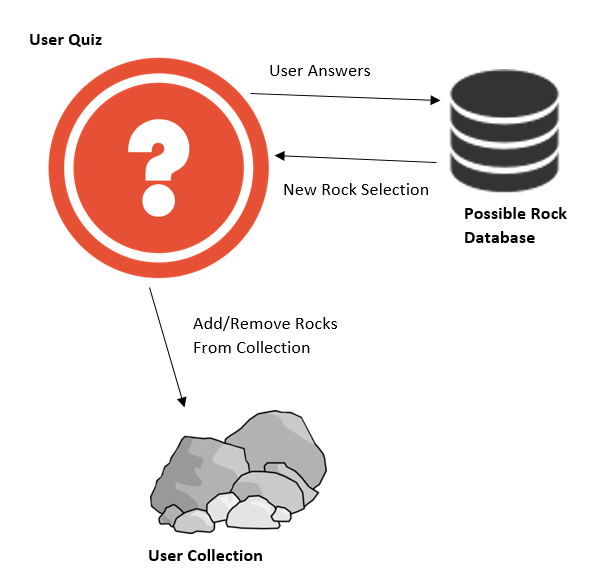
\includegraphics{Interaction.png}

\subsubsection{Constraints}

\begin{itemize}
\item Possible matches are limited to database space\\
\end{itemize}


\subsubsection{Assumptions and Dependencies}

\begin{itemize}
\item Users have enough space on mobile device to hold the app\\
\item User has enabled GPS function in phone\\
\item Device with application is an android phone\\
\end{itemize}


\subsubsection{Apportioning of Requirements}

Some requirements that may be delayed until future versions:

\begin{itemize}
\item Interacting with other users rock collections, such as viewing, and requesting to purchase \\
\item Messaging system between collectors \\
\end{itemize}

\end{document}